\section{Results}
After running our hybrid decision tree algorithm over the various settings of training, tuning, and testing sets, we generate learning curves to compare the performance of standard decision trees (in which a leaf's associated prediction is based on a plurality of the subset of training data at that leaf) and our hybrid trees.  In Figure \ref{fig:learn_curve}, we can see that the performance of standard trees actually fell off with increased training set size, which provides evidence of overfitting. The hybrid trees, in contrast, showed great improvements in accuracy relative to the standard trees, with the margin increasing for larger training and tuning sets.

\begin{figure}
	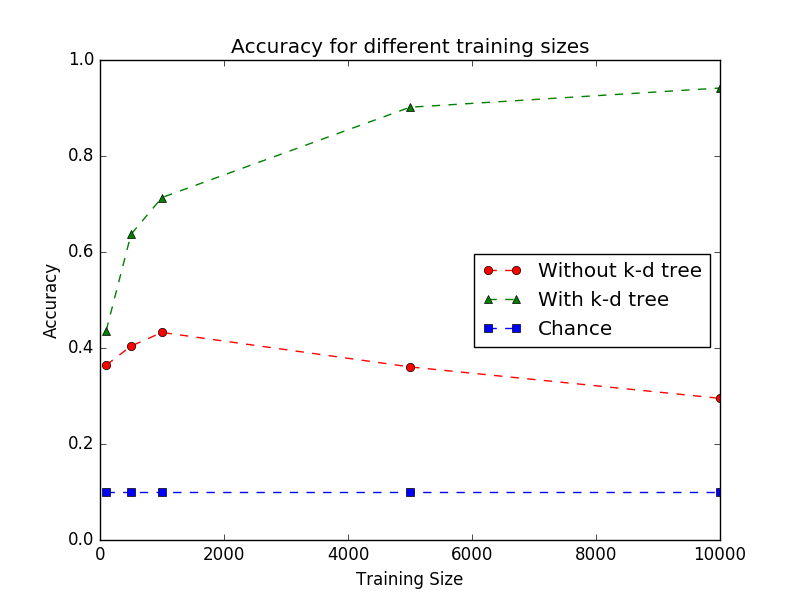
\includegraphics[width=\linewidth]{Figures/learning_curve.png}
	\caption{Learning curve for standard decision trees and hybrid trees with k-d trees.  Note that the chance line assumes a uniform distribution of the 10 handwritten digits.}
	\label{fig:learn_curve}
\end{figure}

To assess the classifier's performance for each handwritten digit, we used the predictions from the setting with 10000 training examples (1000 tuning examples and 10000 testing) to generate a confusion matrix and calculate the values of precision and recall for each digit.  Again, we repeated this for both standard and hybrid decision trees.

\begin{table}
	\begin{tabular}{l|llllllllll}
		&   '0' &   '1' &   '2' &   '3' &   '4' &   '5' &   '6' &   '7' &   '8' &   '9' \\
		\hline
		'0' &   368 &     3 &     2 &     0 &     1 &     4 &     3 &     2 &     0 &     2 \\
		'1' &   517 &  1128 &   444 &   968 &    87 &   742 &   146 &   133 &   866 &    87 \\
		'2' &     8 &     0 &     0 &     0 &     0 &     0 &     0 &     0 &     0 &     0 \\
		'3' &     0 &     0 &     0 &     1 &     0 &     0 &     0 &     0 &     0 &     0 \\
		'4' &     4 &     0 &     1 &     0 &     1 &     0 &     0 &     0 &     3 &     0 \\
		'5' &     8 &     0 &     0 &     2 &     0 &     1 &     0 &     0 &     0 &     0 \\
		'6' &    42 &     4 &   536 &    21 &    18 &    45 &   561 &     5 &    17 &     3 \\
		'7' &    33 &     0 &    49 &    18 &   874 &   100 &   248 &   888 &    86 &   916 \\
		'8' &     0 &     0 &     0 &     0 &     1 &     0 &     0 &     0 &     2 &     0 \\
		'9' &     0 &     0 &     0 &     0 &     0 &     0 &     0 &     0 &     0 &     1 \\
	\end{tabular}
	\caption{Confusion matrix for standard decision trees.  Note that horizontal indices correspond to the actual labels of the handwritten digits while vertical indices correspond to the labels predicted by the tree.}
	\label{table:no_kd_confusion}
\end{table}